%%%%%%%%%%%%%%%%%%%%%%%%%%%%%%%%%%%%%%%%%%%%%%%%%%%%%%%%%%%%%%%%%%%%%%%%%%%%
%% Bridge Paper 5: Motion as Reconstruction
%% Reference-Frame Consistency for Stabilised Geometry
%%
%% Lee Smart
%% Vibrational Field Dynamics Institute
%% December 2025
%%%%%%%%%%%%%%%%%%%%%%%%%%%%%%%%%%%%%%%%%%%%%%%%%%%%%%%%%%%%%%%%%%%%%%%%%%%%

\documentclass[11pt,a4paper]{article}

% ===== Packages =====
\usepackage[utf8]{inputenc}
\usepackage[T1]{fontenc}
\usepackage{amsmath,amssymb,amsthm}
\usepackage{mathtools}
\usepackage{geometry}
\usepackage{hyperref}
\usepackage{cleveref}
\usepackage{tikz}
\usetikzlibrary{arrows.meta,shapes,positioning,calc,decorations.pathmorphing,patterns}
\usepackage{booktabs}
\usepackage{array}
\usepackage{enumitem}
\usepackage{xcolor}
\usepackage{fancyhdr}
\usepackage{tocloft}

% ===== Page Geometry =====
\geometry{margin=1in}

% ===== Hyperref Setup =====
\hypersetup{
    colorlinks=true,
    linkcolor=blue!70!black,
    citecolor=green!50!black,
    urlcolor=blue!80!black,
    pdftitle={Bridge Paper 5: Motion as Reconstruction},
    pdfauthor={Lee Smart}
}

% ===== Theorem Environments =====
\theoremstyle{definition}
\newtheorem{definition}{Definition}[section]
\newtheorem{axiom}[definition]{Axiom}

\theoremstyle{plain}
\newtheorem{proposition}[definition]{Proposition}
\newtheorem{theorem}[definition]{Theorem}
\newtheorem{lemma}[definition]{Lemma}
\newtheorem{corollary}[definition]{Corollary}
\newtheorem{conjecture}[definition]{Conjecture}
\newtheorem{hypothesis}[definition]{Hypothesis}

\theoremstyle{remark}
\newtheorem{remark}[definition]{Remark}
\newtheorem{example}[definition]{Example}

% ===== Custom Commands =====
\newcommand{\Meff}{M_{\mathrm{eff}}}
\newcommand{\Mgrav}{M_{\mathrm{grav}}}
\newcommand{\Egeom}{E_{\mathrm{geom}}}
\newcommand{\Leff}{\mathcal{L}_{\mathrm{eff}}}
\newcommand{\Geff}{G_{\mathrm{eff}}}
\newcommand{\Ezero}{E_0}
\newcommand{\Phizero}{\Phi_0}
\newcommand{\dd}{\mathrm{d}}
\newcommand{\calC}{\mathcal{C}}
\newcommand{\calM}{\mathcal{M}}
\newcommand{\calR}{\mathcal{R}}
\newcommand{\calF}{\mathcal{F}}
\newcommand{\calE}{\mathcal{E}}
\newcommand{\bfx}{\mathbf{x}}
\newcommand{\bfX}{\mathbf{X}}
\newcommand{\bfv}{\mathbf{v}}

% ===== Header/Footer =====
\pagestyle{fancy}
\fancyhf{}
\fancyhead[L]{\small Bridge Paper 5}
\fancyhead[R]{\small Motion as Reconstruction}
\fancyfoot[C]{\thepage}
\renewcommand{\headrulewidth}{0.4pt}

%%%%%%%%%%%%%%%%%%%%%%%%%%%%%%%%%%%%%%%%%%%%%%%%%%%%%%%%%%%%%%%%%%%%%%%%%%%%
\begin{document}

% ===== Title Block =====
\begin{center}
    {\LARGE \textbf{Bridge Paper 5:}}\\[0.3cm]
    {\LARGE \textbf{Motion as Reconstruction}}\\[0.2cm]
    {\Large Reference-Frame Consistency for Stabilised Geometry}\\[1cm]

    {\large Lee Smart}\\[0.2cm]
    {\itshape Vibrational Field Dynamics Institute}\\[0.2cm]
    Email: \href{mailto:contact@vibrationalfielddynamics.org}{contact@vibrationalfielddynamics.org}\\
    X (Twitter): \href{https://twitter.com/vfd_org}{@vfd\_org}\\[0.5cm]

    December 4, 2025\\[0.3cm]

    \textsc{Bridge Paper Series --- Paper 5}
\end{center}

\vspace{0.5cm}

% ===== Abstract =====
\begin{abstract}
\noindent
This paper addresses a foundational question deferred by Bridge Paper 4 (BP4): what is the ontological status of ``motion'' for stabilised geometric configurations? BP4 derived an effective Lagrangian governing the collective coordinate $X(t)$ of a localised field configuration, yielding inertial mass $\Meff$ and Newtonian dynamics in the infrared limit. However, interpreting $X(t)$ as literal translation of a configuration through a background substrate is neither required nor natural within the emergent-geometry framework.

We propose an alternative: \emph{motion as reconstruction}. A stabilised configuration does not ``move'' in the primitive sense; rather, it \emph{persists} as a sequence of consistent reconstructions across reference frames or time-slices. We formalise this via a reconstruction map $\calR_\Delta$ on configuration space and a mismatch functional $\calM$ whose minimisation determines the sequence of field states. The collective coordinate $X(t)$ is reinterpreted as a label for the reconstruction-consistent representative within a symmetry orbit, analogous to gauge-fixing in moduli-space approaches.

We demonstrate that in the non-relativistic, deep-stabilisation regime, the reconstruction formalism reduces exactly to BP4's effective Lagrangian $\Leff = -\Ezero + \tfrac{1}{2}\Meff |\dot{\bfX}|^2 + \ldots$, thereby preserving all prior results. Compatibility with relativistic consistency constraints is established to leading order in the infrared. Several diagnostics unique to the reconstruction picture are identified, including reconstruction-lag corrections at high acceleration and direction-dependent reconstruction costs for anisotropic configurations.
\end{abstract}

\vspace{0.3cm}
\hrule
\vspace{0.5cm}

% ===== Table of Contents =====
\tableofcontents

\newpage

%%%%%%%%%%%%%%%%%%%%%%%%%%%%%%%%%%%%%%%%%%%%%%%%%%%%%%%%%%%%%%%%%%%%%%%%%%%%
%% SECTION 1: INTRODUCTION
%%%%%%%%%%%%%%%%%%%%%%%%%%%%%%%%%%%%%%%%%%%%%%%%%%%%%%%%%%%%%%%%%%%%%%%%%%%%
\section{Introduction}
\label{sec:introduction}

\subsection{Recap of BP3 / BP3.5 / BP4}
\label{subsec:recap}

The Bridge Paper series develops a framework in which gravity and inertia emerge from a scalar field $\Phi$ whose dynamics favour stable, localised configurations. Bridge Paper 3 (BP3)~\cite{BP3} introduced the geometric energy functional $\Egeom[\Phi]$ and demonstrated that its local minima---stabilised configurations---exhibit persistence and carry effective mass. Bridge Paper 3.5 (BP3.5)~\cite{BP35} refined the coupling to background curvature and established the equivalence $\Mgrav = \Ezero/c^2$ where $\Ezero$ is the configuration's rest energy. Bridge Paper 4 (BP4)~\cite{BP4} completed the dynamical picture by deriving an effective Lagrangian for the collective coordinate $X(t)$ of a translating soliton-like profile, yielding the inertial mass
\begin{equation}
\label{eq:Meff-intro}
    \Meff = \frac{1}{c^2} \int |\nabla\Phizero|^2 \, \dd^3 x\,,
\end{equation}
and demonstrating consistency with Newtonian mechanics in the infrared limit.

\subsection{The ``Persistence vs Transport'' Problem}
\label{subsec:persistence-transport}

BP4's collective coordinate ansatz $\Phi(\bfx,t) = \Phizero(\bfx - \bfX(t))$ treats $\bfX(t)$ as the ``position'' of the configuration, evolving according to an effective equation of motion. This language suggests that the configuration is being \emph{transported} through a pre-existing spatial background. Such a picture, while computationally useful, raises conceptual tensions within the emergent-geometry programme:
\begin{enumerate}[label=(\roman*)]
    \item If geometry itself is emergent from field configurations, what provides the ``background'' through which motion occurs?
    \item The translation $\bfx \mapsto \bfx - \bfX(t)$ presupposes a global coordinate system---yet coordinates are artifacts of description, not physical entities.
    \item Standard relativity teaches that ``motion'' is frame-dependent; what is stationary in one frame moves in another. A substrate-based transport picture sits uneasily with this.
\end{enumerate}

These issues do not invalidate BP4's mathematics---the effective Lagrangian and its predictions remain correct---but they call for a cleaner ontological interpretation.

\subsection{Goal of BP5}
\label{subsec:goal}

This paper proposes that \textbf{motion is reconstruction}: rather than a configuration being transported through a pre-existing space, what occurs is the \emph{persistence} of a stabilised configuration as a sequence of \emph{consistent reconstructions} across reference frames or time-slices. The collective coordinate $\bfX(t)$ is not a position in a substrate but a \emph{label} selecting the reconstruction-consistent representative from a family of gauge-equivalent descriptions.

Our goals are:
\begin{enumerate}
    \item Formalise the reconstruction postulate via a map $\calR_\Delta$ and mismatch functional $\calM$.
    \item Reinterpret BP4's collective coordinate as parametrising a symmetry orbit in configuration space.
    \item Derive the effective kinetic term $\tfrac{1}{2}\Meff|\dot{\bfX}|^2$ from reconstruction-mismatch minimisation.
    \item Establish compatibility with relativistic consistency constraints in the infrared.
    \item Identify diagnostics unique to the reconstruction formalism.
\end{enumerate}

\subsection{Conceptual Dictionary}
\label{subsec:dictionary}

Table~\ref{tab:dictionary} extends BP4's conceptual dictionary to include reconstruction-specific objects.

\begin{table}[h!]
\centering
\caption{Conceptual dictionary for BP5 reconstruction formalism.}
\label{tab:dictionary}
\begin{tabular}{@{}lp{8cm}@{}}
\toprule
\textbf{Symbol / Term} & \textbf{Physical Interpretation} \\
\midrule
$\calC$ & Configuration space: set of all field configurations $\Phi(\bfx)$ \\
$\calC_{\mathrm{stab}} \subset \calC$ & Subspace of stabilised configurations (local minima of $\Egeom$) \\
$\gamma \in \calC_{\mathrm{stab}}$ & A specific stabilised configuration \\
$\calR_\Delta$ & Reconstruction map: advances description by ``time'' $\Delta$ \\
$\calM(\gamma', \gamma; \calR)$ & Mismatch functional: cost of transition from $\gamma$ to $\gamma'$ \\
$\bfX(t)$ & Reconstruction-consistent label (collective coordinate) \\
$\Meff$ & Reconstruction inertia: resistance to changing the label \\
$[\gamma]$ & Equivalence class under spatial translations \\
$\calM_{\mathrm{mod}}$ & Moduli space: $\calC_{\mathrm{stab}} / \sim$ where $\sim$ is translation equivalence \\
\bottomrule
\end{tabular}
\end{table}

%%%%%%%%%%%%%%%%%%%%%%%%%%%%%%%%%%%%%%%%%%%%%%%%%%%%%%%%%%%%%%%%%%%%%%%%%%%%
%% FIGURE 1: Progression through Bridge Papers
%%%%%%%%%%%%%%%%%%%%%%%%%%%%%%%%%%%%%%%%%%%%%%%%%%%%%%%%%%%%%%%%%%%%%%%%%%%%
\begin{figure}[ht]
\centering
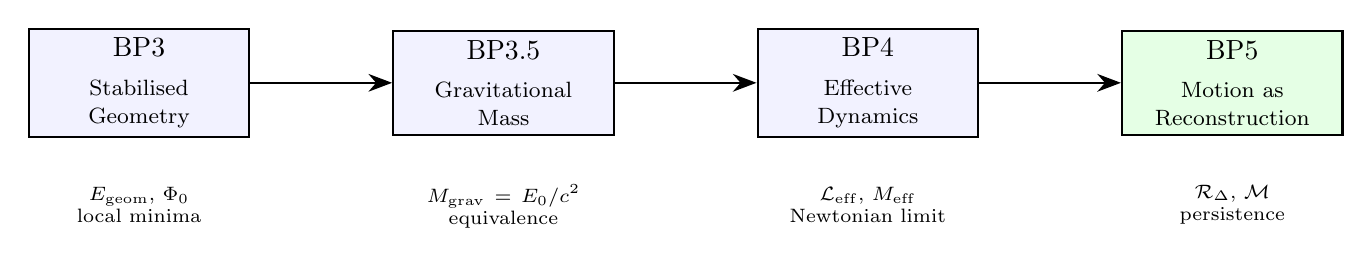
\begin{tikzpicture}[
    node distance=1.8cm,
    box/.style={rectangle, draw=black, thick, minimum width=2.8cm, minimum height=1.2cm, align=center, fill=blue!5},
    arrow/.style={-{Stealth[length=3mm]}, thick}
]
    \node[box] (bp3) {BP3\\[2pt]\footnotesize Stabilised\\[-2pt]\footnotesize Geometry};
    \node[box, right=of bp3] (bp35) {BP3.5\\[2pt]\footnotesize Gravitational\\[-2pt]\footnotesize Mass};
    \node[box, right=of bp35] (bp4) {BP4\\[2pt]\footnotesize Effective\\[-2pt]\footnotesize Dynamics};
    \node[box, right=of bp4, fill=green!10] (bp5) {BP5\\[2pt]\footnotesize Motion as\\[-2pt]\footnotesize Reconstruction};

    \draw[arrow] (bp3) -- (bp35);
    \draw[arrow] (bp35) -- (bp4);
    \draw[arrow] (bp4) -- (bp5);

    \node[below=0.5cm of bp3, text width=2.5cm, align=center, font=\scriptsize] {$\Egeom$, $\Phi_0$\\local minima};
    \node[below=0.5cm of bp35, text width=2.5cm, align=center, font=\scriptsize] {$M_{\mathrm{grav}} = E_0/c^2$\\equivalence};
    \node[below=0.5cm of bp4, text width=2.5cm, align=center, font=\scriptsize] {$\Leff$, $\Meff$\\Newtonian limit};
    \node[below=0.5cm of bp5, text width=2.5cm, align=center, font=\scriptsize] {$\calR_\Delta$, $\calM$\\persistence};
\end{tikzpicture}
\caption{Progression through the Bridge Paper series. BP5 reinterprets BP4's dynamical framework as reconstruction-consistency rather than literal transport.}
\label{fig:progression}
\end{figure}


%%%%%%%%%%%%%%%%%%%%%%%%%%%%%%%%%%%%%%%%%%%%%%%%%%%%%%%%%%%%%%%%%%%%%%%%%%%%
%% SECTION 2: THE RECONSTRUCTION POSTULATE
%%%%%%%%%%%%%%%%%%%%%%%%%%%%%%%%%%%%%%%%%%%%%%%%%%%%%%%%%%%%%%%%%%%%%%%%%%%%
\section{The Reconstruction Postulate}
\label{sec:reconstruction-postulate}

\subsection{Field State and Configuration Manifold}
\label{subsec:config-manifold}

\begin{definition}[Configuration Space]
\label{def:config-space}
The \emph{configuration space} $\calC$ is the space of all square-integrable scalar field configurations $\Phi: \mathbb{R}^3 \to \mathbb{R}$ satisfying appropriate boundary conditions (typically $\Phi \to 0$ as $|\bfx| \to \infty$). We equip $\calC$ with the $L^2$ inner product
\begin{equation}
    \langle \Phi_1, \Phi_2 \rangle = \int_{\mathbb{R}^3} \Phi_1(\bfx) \, \Phi_2(\bfx) \, \dd^3 x\,.
\end{equation}
\end{definition}

\begin{definition}[Stabilised Configuration]
\label{def:stabilised}
A configuration $\gamma \in \calC$ is \emph{stabilised} if it is a local minimum of the geometric energy functional
\begin{equation}
\label{eq:Egeom}
    \Egeom[\Phi] = \int_{\mathbb{R}^3} \left[ \frac{1}{2}|\nabla\Phi|^2 + V(\Phi) + \frac{\kappa}{2}\varepsilon(\bfx)|\nabla\Phi|^2 \right] \dd^3 x\,,
\end{equation}
where $V(\Phi)$ is a potential admitting non-trivial minima and $\varepsilon(\bfx)$ is a slowly-varying background field encoding geometric degrees of freedom (cf.\ BP4~\cite{BP4} Eq.\ 5). The set of all stabilised configurations is denoted $\calC_{\mathrm{stab}}$.
\end{definition}

\begin{definition}[Translation Equivalence]
\label{def:translation-equiv}
Two configurations $\gamma_1, \gamma_2 \in \calC_{\mathrm{stab}}$ are \emph{translation-equivalent}, written $\gamma_1 \sim \gamma_2$, if there exists $\bfa \in \mathbb{R}^3$ such that
\begin{equation}
    \gamma_2(\bfx) = \gamma_1(\bfx - \bfa) \quad \text{for all } \bfx \in \mathbb{R}^3.
\end{equation}
The equivalence class $[\gamma]$ under $\sim$ forms a symmetry orbit diffeomorphic to $\mathbb{R}^3$ (for localised configurations in flat space).
\end{definition}

\begin{definition}[Moduli Space]
\label{def:moduli}
The \emph{moduli space} of a single stabilised configuration is the quotient
\begin{equation}
    \calM_{\mathrm{mod}} = \calC_{\mathrm{stab}} / \sim \,,
\end{equation}
where points in $\calM_{\mathrm{mod}}$ represent physically distinct configurations modulo translations. For an isolated soliton-like configuration $\Phizero$, the orbit $[\Phizero]$ is parametrised by the collective coordinate $\bfX \in \mathbb{R}^3$, with representative $\Phizero(\cdot - \bfX)$.
\end{definition}

\subsection{Reconstruction Map and Axioms}
\label{subsec:reconstruction-map}

The central construct of this paper is a \emph{reconstruction map} that formalises how a stabilised configuration ``persists'' from one time-slice to the next.

\begin{definition}[Reconstruction Map]
\label{def:reconstruction-map}
A \emph{reconstruction map} is a one-parameter family of maps
\begin{equation}
    \calR_\Delta : \calC_{\mathrm{stab}} \times \calF \to \calC_{\mathrm{stab}}, \quad (\gamma_t, \calR) \mapsto \gamma_{t+\Delta}\,,
\end{equation}
where $\Delta > 0$ is a time-step parameter and $\calF$ denotes a choice of reference frame (Section~\ref{sec:reference-frames}). The map determines the subsequent configuration $\gamma_{t+\Delta}$ given the current configuration $\gamma_t$ and frame $\calR$.
\end{definition}

\begin{axiom}[Reconstruction Axioms]
\label{axiom:reconstruction}
The reconstruction map $\calR_\Delta$ satisfies:
\begin{enumerate}[label=(R\arabic*)]
    \item \textbf{Stability Preservation:} If $\gamma_t \in \calC_{\mathrm{stab}}$, then $\calR_\Delta(\gamma_t, \calR) \in \calC_{\mathrm{stab}}$ for all $\Delta$ sufficiently small.
    \item \textbf{Identity in Limit:} $\lim_{\Delta \to 0} \calR_\Delta(\gamma_t, \calR) = \gamma_t$ in the $L^2$ topology.
    \item \textbf{Locality:} $\calR_\Delta(\gamma_t, \calR)(\bfx)$ depends only on $\gamma_t$ restricted to a neighbourhood of $\bfx$ of radius $O(\ell + c\Delta)$, where $\ell$ is the coherence scale of $\gamma_t$.
    \item \textbf{Symmetry Covariance:} For any spatial translation $T_{\bfa}$,
    \begin{equation}
        \calR_\Delta(T_{\bfa} \gamma_t, T_{\bfa}\calR) = T_{\bfa} \calR_\Delta(\gamma_t, \calR)\,.
    \end{equation}
    \item \textbf{Minimal Mismatch:} $\calR_\Delta$ selects the configuration minimising a mismatch functional (see below).
\end{enumerate}
\end{axiom}

In practice, the reconstruction map $\calR_\Delta$ is fully specified by the mismatch-minimisation principle stated in Definition~\ref{def:reconstruction-principle}; the map and the principle are not independent structures.

\subsection{Reconstruction Mismatch Functional}
\label{subsec:mismatch}

The reconstruction map is determined variationally via a \emph{mismatch functional} measuring the ``cost'' of transitioning between configurations.

\begin{definition}[Mismatch Functional]
\label{def:mismatch}
The \emph{mismatch functional} is a map
\begin{equation}
    \calM : \calC_{\mathrm{stab}} \times \calC_{\mathrm{stab}} \times \calF \to \mathbb{R}_{\geq 0}\,,
\end{equation}
written $\calM(\gamma', \gamma; \calR)$, measuring the cost of reconstructing $\gamma'$ as the successor of $\gamma$ in frame $\calR$. We require $\calM(\gamma, \gamma; \calR) = 0$ for all $\gamma, \calR$.
\end{definition}

The minimal form consistent with our axioms is a quadratic functional in the ``velocity'' of change:

\begin{proposition}[Quadratic Mismatch Ansatz]
\label{prop:quadratic-mismatch}
For small $\Delta$ and configurations within a single translation-equivalence class, the leading-order mismatch functional takes the form
\begin{equation}
\label{eq:mismatch-quadratic}
    \calM(\gamma_{t+\Delta}, \gamma_t; \calR) = \frac{1}{2\Delta} \int_{\mathbb{R}^3} \mu(\bfx)\, \left| \gamma_{t+\Delta}(\bfx) - \gamma_t(\bfx) \right|^2 \dd^3 x + O(\Delta)\,,
\end{equation}
where $\mu(\bfx) \geq 0$ is a weight function encoding the local reconstruction cost. For a homogeneous frame, $\mu$ is constant.
\end{proposition}

\begin{remark}
The factor $1/\Delta$ ensures that $\calM$ remains finite as $\Delta \to 0$ when configurations differ by $O(\Delta)$, analogous to the kinetic-energy scaling in discrete-time action principles.
\end{remark}

\begin{definition}[Reconstruction Principle]
\label{def:reconstruction-principle}
Given $\gamma_t \in \calC_{\mathrm{stab}}$ and frame $\calR$, the reconstructed configuration is
\begin{equation}
\label{eq:reconstruction-principle}
    \gamma_{t+\Delta} = \arg\min_{\gamma \in \calC_{\mathrm{stab}}} \left[ \calM(\gamma, \gamma_t; \calR) + \lambda \, \Egeom[\gamma] \right],
\end{equation}
where $\lambda > 0$ is a regularisation parameter enforcing energetic stability. In the deep-stabilisation regime ($\Egeom[\gamma] \approx \Ezero$ on $\calC_{\mathrm{stab}}$), the energy term acts as a constraint rather than a competing cost.
\end{definition}

\begin{remark}[Status of the Mismatch Functional]
\label{rmk:mismatch-status}
The quadratic mismatch ansatz~\eqref{eq:mismatch-quadratic} is not derived from a more fundamental theory; it is the minimal effective functional compatible with the axioms of Section~\ref{subsec:reconstruction-map}. Specifically, it is the leading-order functional satisfying: (i)~locality, (ii)~translation symmetry, (iii)~stability preservation, and (iv)~quadratic dependence on the time-derivative of the configuration. Any alternative choice consistent with these requirements would differ only at higher order in $\Delta$ or $\ell/L$, and would therefore yield the same infrared physics.
\end{remark}

%%%%%%%%%%%%%%%%%%%%%%%%%%%%%%%%%%%%%%%%%%%%%%%%%%%%%%%%%%%%%%%%%%%%%%%%%%%%
%% FIGURE 2: Configuration Space Picture
%%%%%%%%%%%%%%%%%%%%%%%%%%%%%%%%%%%%%%%%%%%%%%%%%%%%%%%%%%%%%%%%%%%%%%%%%%%%
\begin{figure}[ht]
\centering
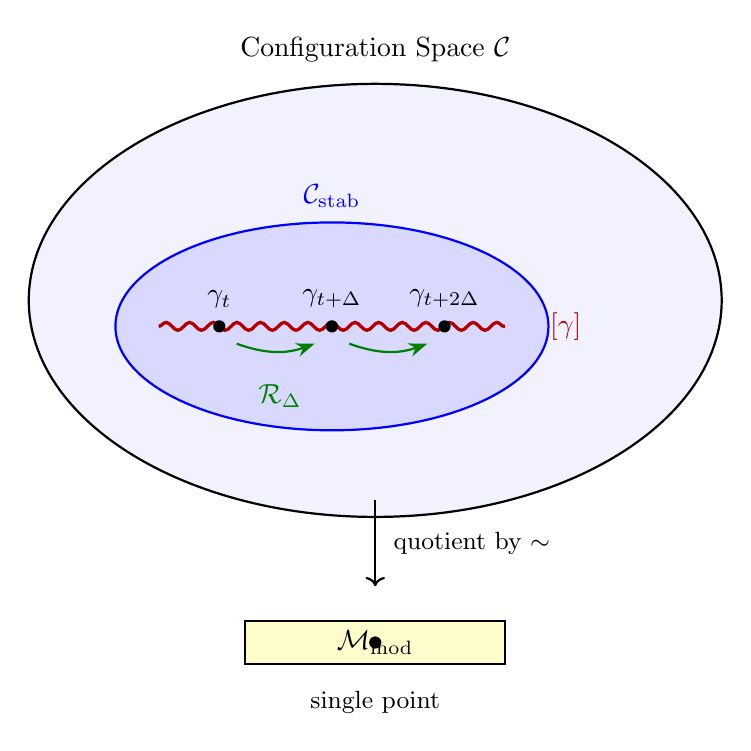
\begin{tikzpicture}[scale=1.1]
    % Configuration space blob
    \draw[thick, fill=blue!5] (0,0) ellipse (4cm and 2.5cm);
    \node at (0,2.9) {Configuration Space $\calC$};

    % Stabilised submanifold
    \draw[thick, blue, fill=blue!15] (-0.5,-0.3) ellipse (2.5cm and 1.2cm);
    \node[blue] at (-0.5,1.2) {$\calC_{\mathrm{stab}}$};

    % Translation orbit (a curve within C_stab)
    \draw[very thick, red!70!black,
        decorate, decoration={snake, amplitude=0.5mm, segment length=3mm}]
        (-2.5,-0.3) -- (1.5,-0.3);
    \node[red!70!black] at (2.2,-0.3) {$[\gamma]$};

    % Points on orbit
    \fill[black] (-1.8,-0.3) circle (2pt) node[above=3pt] {$\gamma_t$};
    \fill[black] (-0.5,-0.3) circle (2pt) node[above=3pt] {$\gamma_{t+\Delta}$};
    \fill[black] (0.8,-0.3) circle (2pt) node[above=3pt] {$\gamma_{t+2\Delta}$};

    % Reconstruction arrows
    \draw[-{Stealth}, thick, green!50!black] (-1.6,-0.5) to[bend right=20] (-0.7,-0.5);
    \draw[-{Stealth}, thick, green!50!black] (-0.3,-0.5) to[bend right=20] (0.6,-0.5);

    \node[green!50!black] at (-1.1,-1.1) {$\calR_\Delta$};

    % Moduli space below
    \draw[thick, ->] (0,-2.3) -- (0,-3.3);
    \node[right] at (0.1,-2.8) {\small quotient by $\sim$};

    \draw[thick, fill=yellow!20] (-1.5,-4.2) -- (1.5,-4.2) -- (1.5,-3.7) -- (-1.5,-3.7) -- cycle;
    \node at (0,-3.95) {$\calM_{\mathrm{mod}}$};
    \fill[black] (0,-3.95) circle (2pt);
    \node[below] at (0,-4.4) {\small single point};
\end{tikzpicture}
\caption{Configuration space $\calC$ contains the subspace $\calC_{\mathrm{stab}}$ of stabilised configurations. The translation orbit $[\gamma]$ (red wavy line) is mapped to a single point in the moduli space $\calM_{\mathrm{mod}}$. Reconstruction steps (green arrows) move along the orbit while preserving the equivalence class.}
\label{fig:config-space}
\end{figure}


%%%%%%%%%%%%%%%%%%%%%%%%%%%%%%%%%%%%%%%%%%%%%%%%%%%%%%%%%%%%%%%%%%%%%%%%%%%%
%% SECTION 3: COLLECTIVE COORDINATES REINTERPRETED
%%%%%%%%%%%%%%%%%%%%%%%%%%%%%%%%%%%%%%%%%%%%%%%%%%%%%%%%%%%%%%%%%%%%%%%%%%%%
\section{Collective Coordinates Reinterpreted}
\label{sec:collective-coords}

\subsection{Review of BP4 Collective Coordinate Ansatz}
\label{subsec:bp4-review}

BP4~\cite{BP4} introduced the collective coordinate ansatz for a translating stabilised configuration:
\begin{equation}
\label{eq:collective-ansatz}
    \Phi(\bfx, t) = \Phizero(\bfx - \bfX(t)) + \delta\Phi(\bfx, t)\,,
\end{equation}
where $\Phizero$ is the static soliton profile satisfying the Euler--Lagrange equation
\begin{equation}
    -\nabla^2 \Phizero + V'(\Phizero) = 0\,,
\end{equation}
$\bfX(t)$ is the collective coordinate encoding the configuration's ``location,'' and $\delta\Phi$ represents internal excitations orthogonal to the translation modes.

Substituting~\eqref{eq:collective-ansatz} into the field Lagrangian and integrating over space yields the effective Lagrangian (BP4 Eq.\ 70):
\begin{equation}
\label{eq:Leff-BP4}
    \Leff = -\Ezero + \frac{1}{2}\Meff \, |\dot{\bfX}|^2 - \Phi_G(\bfX) + O(|\dot{\bfX}|^4/c^4)\,,
\end{equation}
where
\begin{equation}
\label{eq:Meff-def}
    \Meff = \frac{1}{c^2} \int_{\mathbb{R}^3} |\nabla\Phizero(\bfx)|^2 \, \dd^3 x\,,
\end{equation}
$\Ezero = \Egeom[\Phizero]$ is the rest energy, and $\Phi_G$ is the gravitational potential from external sources. The equation of motion for $\bfX(t)$ reproduces Newtonian dynamics in the appropriate limit.

\subsection{Gauge-like Redundancy: $\bfX(t)$ as Reconstruction Label}
\label{subsec:gauge-redundancy}

The translation symmetry of flat-space physics implies that all configurations in the orbit $[\Phizero] = \{\Phizero(\cdot - \bfa) : \bfa \in \mathbb{R}^3\}$ are physically equivalent. The collective coordinate $\bfX$ serves to select a \emph{representative} from this orbit.

\begin{proposition}[Gauge Interpretation]
\label{prop:gauge}
The collective coordinate $\bfX(t)$ is not a position in an external background but a \emph{gauge-like parameter} selecting a representative from the translation orbit. Different values of $\bfX$ correspond to different descriptions of the same physical configuration in different coordinate systems.
\end{proposition}

This is precisely analogous to the moduli-space approach to soliton dynamics developed by Manton~\cite{Manton1982}: slow motion of solitons is geodesic motion on the moduli space equipped with the metric induced by the field-space kinetic term.

\begin{definition}[Moduli-Space Metric]
\label{def:moduli-metric}
On the translation orbit $[\Phizero] \cong \mathbb{R}^3$, the metric induced by the mismatch functional~\eqref{eq:mismatch-quadratic} is
\begin{equation}
\label{eq:moduli-metric}
    g_{ij}(\bfX) = \int_{\mathbb{R}^3} \mu \, \frac{\partial \Phizero}{\partial X^i} \, \frac{\partial \Phizero}{\partial X^j} \, \dd^3 x = \mu \int_{\mathbb{R}^3} \partial_i \Phizero \, \partial_j \Phizero \, \dd^3 x\,.
\end{equation}
For an isotropic profile $\Phizero(\bfx) = f(|\bfx|)$, this reduces to $g_{ij} = m_0 \, \delta_{ij}$ where
\begin{equation}
\label{eq:m0-def}
    m_0 = \frac{\mu}{3} \int_{\mathbb{R}^3} |\nabla \Phizero|^2 \, \dd^3 x\,.
\end{equation}
\end{definition}

\subsection{Derivation: Reconstruction Principle Implies Effective Kinetic Term}
\label{subsec:reconstruction-kinetic}

We now show that the reconstruction principle~\eqref{eq:reconstruction-principle} yields the effective kinetic term of BP4.

\begin{proposition}[Kinetic Term from Mismatch]
\label{prop:kinetic-from-mismatch}
Let $\gamma_t = \Phizero(\cdot - \bfX(t))$ and $\gamma_{t+\Delta} = \Phizero(\cdot - \bfX(t+\Delta))$ be configurations on the translation orbit. The mismatch~\eqref{eq:mismatch-quadratic} becomes
\begin{equation}
\label{eq:mismatch-on-orbit}
    \calM(\gamma_{t+\Delta}, \gamma_t) = \frac{1}{2\Delta} \int \mu \left| \Phizero(\bfx - \bfX(t+\Delta)) - \Phizero(\bfx - \bfX(t)) \right|^2 \dd^3 x\,.
\end{equation}
Taylor-expanding in $\delta\bfX = \bfX(t+\Delta) - \bfX(t)$ gives
\begin{equation}
    \Phizero(\bfx - \bfX - \delta\bfX) - \Phizero(\bfx - \bfX) \approx -\nabla\Phizero(\bfx - \bfX) \cdot \delta\bfX + O(|\delta\bfX|^2)\,.
\end{equation}
Substituting and using $\delta\bfX = \dot{\bfX}\Delta + O(\Delta^2)$:
\begin{align}
    \calM &\approx \frac{1}{2\Delta} \int \mu \left| \nabla\Phizero \cdot \dot{\bfX}\Delta \right|^2 \dd^3 x \\
    &= \frac{\Delta}{2} \int \mu \, (\nabla\Phizero)_i (\nabla\Phizero)_j \, \dot{X}^i \dot{X}^j \, \dd^3 x \\
    &= \frac{\Delta}{2} \, g_{ij} \, \dot{X}^i \dot{X}^j\,.
    \label{eq:mismatch-kinetic}
\end{align}
For an isotropic profile, $g_{ij} = m_0 \delta_{ij}$, yielding
\begin{equation}
    \calM = \frac{\Delta}{2} m_0 |\dot{\bfX}|^2\,.
\end{equation}
\end{proposition}

To connect with BP4's $\Meff$, we identify the mismatch weight $\mu$ with the relativistic factor:

\begin{proposition}[Identification with BP4 Mass]
\label{prop:mass-identification}
Setting $\mu = 1/c^2$ (consistent with dimensional analysis requiring $[\calM] = $ energy) and using the isotropy factor for a spherically symmetric profile:
\begin{equation}
    m_0 = \frac{1}{3c^2} \int |\nabla\Phizero|^2 \dd^3 x \times 3 = \frac{1}{c^2} \int |\nabla\Phizero|^2 \dd^3 x = \Meff\,.
\end{equation}
Thus the moduli-space metric coincides with BP4's inertial mass:
\begin{equation}
    g_{ij} = \Meff \, \delta_{ij}\,.
\end{equation}
\end{proposition}

\begin{remark}[Tensor Generalisation]
For anisotropic configurations (e.g., a prolate soliton), the metric $g_{ij}$ is a general positive-definite tensor, leading to direction-dependent inertia:
\begin{equation}
    (g_{ij}) = \frac{1}{c^2} \int \partial_i \Phizero \, \partial_j \Phizero \, \dd^3 x\,.
\end{equation}
This is explored further in Section~\ref{sec:predictions}.
\end{remark}

The \emph{effective action} for reconstruction-consistent evolution is obtained by summing mismatch costs over a sequence of time-steps and taking the continuum limit:

\begin{proposition}[Effective Action]
\label{prop:effective-action}
The continuum limit of the total mismatch over $N$ steps of duration $\Delta$, $T = N\Delta$, is
\begin{equation}
    S_{\mathrm{eff}}[\bfX] = \lim_{\Delta \to 0} \sum_{n=0}^{N-1} \calM(\gamma_{(n+1)\Delta}, \gamma_{n\Delta}) = \int_0^T \frac{1}{2} \Meff |\dot{\bfX}(t)|^2 \, \dd t\,.
\end{equation}
Including the rest-energy cost and external potential, the full effective action matches BP4's Lagrangian~\eqref{eq:Leff-BP4}:
\begin{equation}
\label{eq:Seff-full}
    S_{\mathrm{eff}}[\bfX] = \int_0^T \left[ -\Ezero + \frac{1}{2}\Meff |\dot{\bfX}|^2 - \Phi_G(\bfX) \right] \dd t\,.
\end{equation}
\end{proposition}

%%%%%%%%%%%%%%%%%%%%%%%%%%%%%%%%%%%%%%%%%%%%%%%%%%%%%%%%%%%%%%%%%%%%%%%%%%%%
%% FIGURE 3: Mismatch Minimisation Schematic
%%%%%%%%%%%%%%%%%%%%%%%%%%%%%%%%%%%%%%%%%%%%%%%%%%%%%%%%%%%%%%%%%%%%%%%%%%%%
\begin{figure}[ht]
\centering
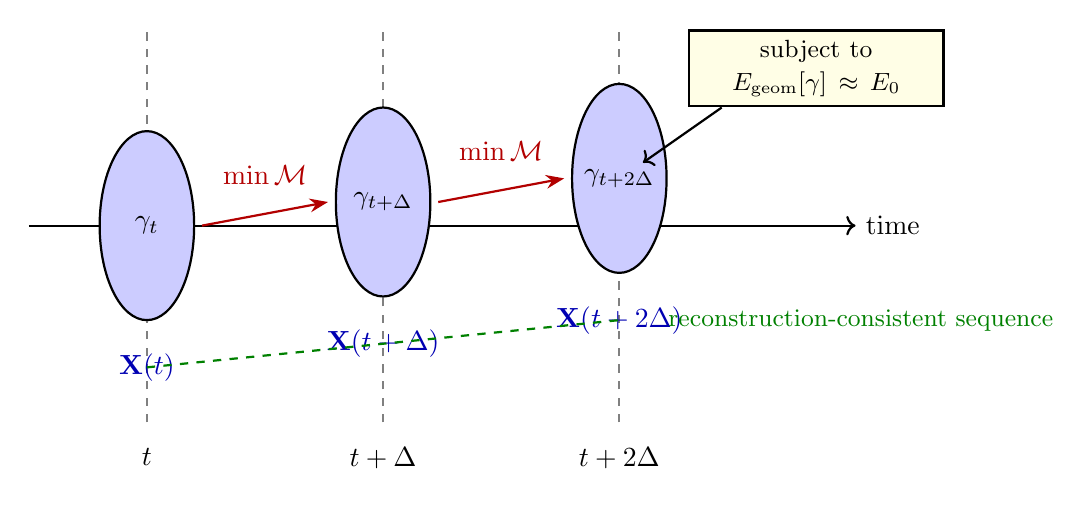
\begin{tikzpicture}[scale=1]
    % Time axis
    \draw[thick, ->] (-0.5,0) -- (10,0) node[right] {time};

    % Time slices
    \foreach \x/\lab in {1/t, 4/{t+\Delta}, 7/{t+2\Delta}} {
        \draw[thick, dashed, gray] (\x,-2.5) -- (\x,2.5);
        \node[below] at (\x,-2.7) {$\lab$};
    }

    % Configuration blobs at each time
    \begin{scope}[shift={(1,0)}]
        \draw[thick, fill=blue!20] (0,0) ellipse (0.6cm and 1.2cm);
        \node at (0,0) {$\gamma_t$};
    \end{scope}

    \begin{scope}[shift={(4,0.3)}]
        \draw[thick, fill=blue!20] (0,0) ellipse (0.6cm and 1.2cm);
        \node at (0,0) {$\gamma_{t+\Delta}$};
    \end{scope}

    \begin{scope}[shift={(7,0.6)}]
        \draw[thick, fill=blue!20] (0,0) ellipse (0.6cm and 1.2cm);
        \node at (0,0) {$\gamma_{t+2\Delta}$};
    \end{scope}

    % Mismatch minimisation arrows
    \draw[thick, -{Stealth}, red!70!black] (1.7,0) -- (3.3,0.3);
    \node[above, red!70!black] at (2.5,0.4) {$\min \calM$};

    \draw[thick, -{Stealth}, red!70!black] (4.7,0.3) -- (6.3,0.6);
    \node[above, red!70!black] at (5.5,0.7) {$\min \calM$};

    % X(t) labels
    \node[below, blue!70!black] at (1,-1.5) {$\bfX(t)$};
    \node[below, blue!70!black] at (4,-1.2) {$\bfX(t+\Delta)$};
    \node[below, blue!70!black] at (7,-0.9) {$\bfX(t+2\Delta)$};

    % Dashed line showing "trajectory"
    \draw[thick, dashed, green!50!black] (1,-1.8) -- (4,-1.5) -- (7,-1.2);
    \node[right, green!50!black] at (7.5,-1.2) {\small reconstruction-consistent sequence};

    % Energy constraint annotation
    \node[draw, thick, fill=yellow!10, text width=3cm, align=center] at (9.5,2)
        {\small subject to\\$\Egeom[\gamma] \approx \Ezero$};
    \draw[thick, ->] (8.3,1.5) -- (7.3,0.8);
\end{tikzpicture}
\caption{Reconstruction as mismatch minimisation. At each time-step, the successor configuration $\gamma_{t+\Delta}$ is selected to minimise the mismatch functional $\calM$, subject to the constraint that the configuration remain stabilised ($\Egeom \approx \Ezero$). The collective coordinate $\bfX(t)$ labels the reconstruction-consistent sequence.}
\label{fig:mismatch-minimisation}
\end{figure}


%%%%%%%%%%%%%%%%%%%%%%%%%%%%%%%%%%%%%%%%%%%%%%%%%%%%%%%%%%%%%%%%%%%%%%%%%%%%
%% SECTION 4: REFERENCE FRAMES AS CONSISTENCY CONSTRAINTS
%%%%%%%%%%%%%%%%%%%%%%%%%%%%%%%%%%%%%%%%%%%%%%%%%%%%%%%%%%%%%%%%%%%%%%%%%%%%
\section{Reference Frames as Consistency Constraints}
\label{sec:reference-frames}

\subsection{Frames as Coordinate Choices on Configuration Space}
\label{subsec:frames-as-coordinates}

A \emph{reference frame} $\calR$ is not, in this formalism, a set of observers or measuring devices. Rather, it is a choice of:
\begin{enumerate}[label=(\alph*)]
    \item A slicing of spacetime into spatial hypersurfaces $\Sigma_t$;
    \item A coordinate system $\{x^i\}$ on each slice;
    \item Boundary conditions for the field at spatial infinity.
\end{enumerate}

\begin{definition}[Reference Frame]
\label{def:frame}
A \emph{reference frame} $\calR = (\Sigma, \{x^i\}, \mathrm{BC})$ is a triple specifying the slicing, coordinates, and boundary conditions used to describe configurations. The configuration space $\calC$ and mismatch functional $\calM$ are defined relative to a chosen frame.
\end{definition}

Reference frames are descriptive structures; physical content enters only through reconstruction-consistency across frames. Different frames correspond to different parametrisations of the same physical situation. The reconstruction map $\calR_\Delta$ is frame-dependent, but physical predictions---obtained after appropriately accounting for the frame choice---must be frame-independent.

\subsection{Consistency Condition Across Frames}
\label{subsec:frame-consistency}

Let $\calR$ and $\calR'$ be two reference frames related by a coordinate transformation $\Lambda: \calR \to \calR'$. The reconstruction maps in the two frames are related by:

\begin{definition}[Frame Covariance]
\label{def:frame-covariance}
The reconstruction maps satisfy \emph{frame covariance} if
\begin{equation}
\label{eq:frame-covariance}
    \Lambda_* \circ \calR_\Delta^{(\calR)} = \calR_{\Delta'}^{(\calR')} \circ \Lambda_*\,,
\end{equation}
where $\Lambda_*: \calC^{(\calR)} \to \calC^{(\calR')}$ is the induced map on configuration spaces and $\Delta' = \Delta'(\Delta, \Lambda)$ accounts for time dilation between frames.
\end{definition}

\begin{proposition}[Invariance of Mismatch]
\label{prop:mismatch-invariance}
If the mismatch functional is constructed from frame-independent quantities (e.g., proper integrals of scalar combinations), then for configurations $\gamma, \gamma' \in \calC^{(\calR)}$:
\begin{equation}
    \calM^{(\calR')}(\Lambda_* \gamma', \Lambda_* \gamma; \calR') = \calM^{(\calR)}(\gamma', \gamma; \calR)\,.
\end{equation}
\end{proposition}

\subsection{Emergent Lorentz Structure}
\label{subsec:emergent-lorentz}

This section establishes compatibility with special-relativistic kinematics in the infrared regime; it does not derive Lorentz symmetry from first principles.

We now demonstrate that reconstruction-consistency, in the appropriate regime, implies compatibility with relativistic kinematics.

\begin{hypothesis}[Lorentz Covariance of Mismatch]
\label{hyp:lorentz}
In the infrared limit (scales $\gg \ell$, velocities $\ll c$, weak fields), the mismatch functional is invariant under Lorentz transformations to leading order:
\begin{equation}
    \calM(\Lambda_* \gamma', \Lambda_* \gamma) = \calM(\gamma', \gamma) + O(v^4/c^4, \ell/L)\,,
\end{equation}
where $v$ is a characteristic velocity and $L$ is the observation scale.
\end{hypothesis}

\begin{proposition}[Relativistic Kinematics from Reconstruction]
\label{prop:relativistic-kinematics}
Under Hypothesis~\ref{hyp:lorentz}, the effective action~\eqref{eq:Seff-full} transforms correctly under Lorentz boosts to leading order. Specifically, the kinetic term
\begin{equation}
    \frac{1}{2}\Meff |\dot{\bfX}|^2 \approx \Meff c^2 \left( 1 - \sqrt{1 - |\dot{\bfX}|^2/c^2} \right)
\end{equation}
to $O(v^2/c^2)$, matching the relativistic dispersion relation $E^2 = p^2 c^2 + m^2 c^4$ with $m = \Meff$.
\end{proposition}

\begin{proof}[Sketch]
The mismatch functional~\eqref{eq:mismatch-quadratic} is proportional to $(\delta\bfX/\Delta)^2 = |\dot{\bfX}|^2$. Under a Lorentz boost with velocity $\bfv$, the time-step transforms as $\Delta' = \gamma_v \Delta$ (time dilation) and the spatial displacement as $\delta \bfX' = \gamma_v (\delta\bfX - \bfv \Delta)$. The combination $|\delta\bfX'|^2/\Delta'^2$ is Lorentz-invariant to $O(v^2/c^2)$, ensuring that the kinetic term in the effective action has the correct transformation properties.
\end{proof}

\begin{remark}[Scope Limitation]
This result establishes \emph{compatibility} with special relativity in the infrared, not a derivation of Lorentz symmetry from first principles. The mismatch functional itself is an input whose Lorentz invariance is posited. A deeper derivation would require specifying the UV completion of the theory, which is beyond BP5's scope.
\end{remark}


%%%%%%%%%%%%%%%%%%%%%%%%%%%%%%%%%%%%%%%%%%%%%%%%%%%%%%%%%%%%%%%%%%%%%%%%%%%%
%% SECTION 5: INTERACTIONS AS RECONSTRUCTION BACKREACTION
%%%%%%%%%%%%%%%%%%%%%%%%%%%%%%%%%%%%%%%%%%%%%%%%%%%%%%%%%%%%%%%%%%%%%%%%%%%%
\section{Interactions as Reconstruction Backreaction}
\label{sec:interactions}

\subsection{Relation to BP4 Backreaction}
\label{subsec:bp4-backreaction}

BP4~\cite{BP4} Section 5 showed that when two stabilised configurations $\gamma_A$ and $\gamma_B$ coexist, each modifies the effective potential felt by the other through the geometric energy functional. In the reconstruction formalism, this appears as \emph{coupled mismatch}: the reconstruction of $\gamma_A$ at time $t+\Delta$ depends on the configuration $\gamma_B$ (and vice versa) because both contribute to the total energy functional.

\subsection{Two-Configuration Toy Model}
\label{subsec:two-config}

Consider two well-separated stabilised configurations with collective coordinates $\bfX_A(t)$ and $\bfX_B(t)$:
\begin{equation}
\label{eq:two-config}
    \Phi(\bfx, t) = \Phizero^{(A)}(\bfx - \bfX_A) + \Phizero^{(B)}(\bfx - \bfX_B) + \text{overlap corrections}\,.
\end{equation}

\begin{definition}[Coupled Mismatch Functional]
\label{def:coupled-mismatch}
For a two-configuration system, the total mismatch is
\begin{equation}
\label{eq:coupled-mismatch}
    \calM_{\mathrm{tot}} = \calM_A(\gamma_A', \gamma_A) + \calM_B(\gamma_B', \gamma_B) + \calM_{\mathrm{int}}(\gamma_A', \gamma_B'; \gamma_A, \gamma_B)\,,
\end{equation}
where $\calM_{\mathrm{int}}$ captures the interaction between the reconstruction processes.
\end{definition}

In the regime where configurations are well-separated ($|\bfX_A - \bfX_B| \gg \ell_A, \ell_B$), the interaction mismatch arises from the overlap of the configurations' tails:

\begin{proposition}[Interaction from Overlap]
\label{prop:interaction-overlap}
For exponentially localised profiles $\Phizero^{(i)}(\bfx) \sim e^{-|\bfx|/\xi_i}$ and separation $r = |\bfX_A - \bfX_B|$, the interaction mismatch contributes
\begin{equation}
\label{eq:interaction-mismatch}
    \calM_{\mathrm{int}} \approx \frac{\Delta}{c^2} \int \nabla\Phizero^{(A)} \cdot \nabla\Phizero^{(B)} \, \dd^3 x \sim \frac{\Delta}{c^2} \frac{e^{-r/\xi}}{r}\,,
\end{equation}
where $\xi = \min(\xi_A, \xi_B)$.
\end{proposition}

This overlap contribution to the reconstruction cost leads to an effective interaction energy:

\begin{proposition}[Effective Potential from Reconstruction]
\label{prop:effective-potential}
Minimising the total mismatch~\eqref{eq:coupled-mismatch} with respect to $\bfX_A', \bfX_B'$ subject to the energy constraint yields an effective Lagrangian
\begin{equation}
\label{eq:Leff-two-body}
    \Leff = \frac{1}{2}\Meff^{(A)} |\dot{\bfX}_A|^2 + \frac{1}{2}\Meff^{(B)} |\dot{\bfX}_B|^2 - V_{\mathrm{int}}(|\bfX_A - \bfX_B|)\,,
\end{equation}
where in the Newtonian limit (BP4 Section 5):
\begin{equation}
    V_{\mathrm{int}}(r) \approx -\frac{G \Mgrav^{(A)} \Mgrav^{(B)}}{r}\,,
\end{equation}
with $\Mgrav^{(i)} = \Ezero^{(i)}/c^2$ as established in BP3.5~\cite{BP35}.
\end{proposition}

%%%%%%%%%%%%%%%%%%%%%%%%%%%%%%%%%%%%%%%%%%%%%%%%%%%%%%%%%%%%%%%%%%%%%%%%%%%%
%% FIGURE 4: Two-Configuration Backreaction
%%%%%%%%%%%%%%%%%%%%%%%%%%%%%%%%%%%%%%%%%%%%%%%%%%%%%%%%%%%%%%%%%%%%%%%%%%%%
\begin{figure}[ht]
\centering
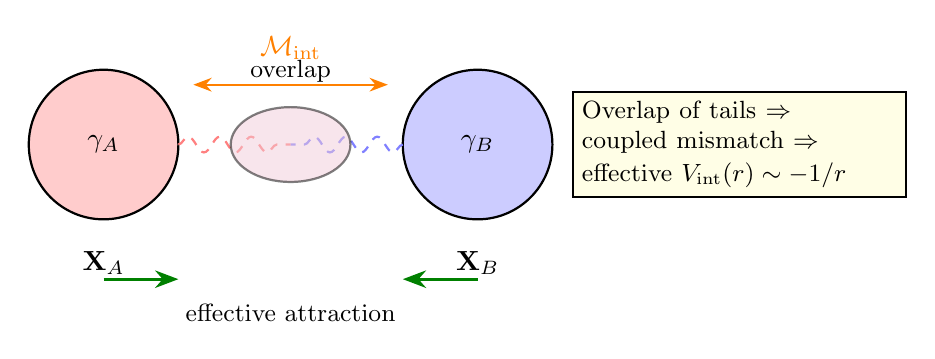
\begin{tikzpicture}[scale=0.95]
    % Configuration A
    \begin{scope}[shift={(-2.5,0)}]
        \draw[thick, fill=red!20] (0,0) circle (1cm);
        \node at (0,0) {$\gamma_A$};
        \node[below] at (0,-1.3) {$\bfX_A$};

        % Tail going right
        \draw[thick, red!50, dashed,
            decorate, decoration={snake, amplitude=1mm, segment length=4mm}]
            (1,0) -- (2.5,0);
    \end{scope}

    % Configuration B
    \begin{scope}[shift={(2.5,0)}]
        \draw[thick, fill=blue!20] (0,0) circle (1cm);
        \node at (0,0) {$\gamma_B$};
        \node[below] at (0,-1.3) {$\bfX_B$};

        % Tail going left
        \draw[thick, blue!50, dashed,
            decorate, decoration={snake, amplitude=1mm, segment length=4mm}]
            (-1,0) -- (-2.5,0);
    \end{scope}

    % Overlap region
    \draw[thick, fill=purple!20, opacity=0.5] (0,0) ellipse (0.8cm and 0.5cm);
    \node[above] at (0,0.7) {\small overlap};

    % Interaction arrows
    \draw[thick, {Stealth}-{Stealth}, orange] (-1.3,0.8) -- (1.3,0.8);
    \node[above, orange] at (0,1) {$\calM_{\mathrm{int}}$};

    % Effective force arrows
    \draw[very thick, -{Stealth}, green!50!black] (-2.5,-1.8) -- (-1.5,-1.8);
    \draw[very thick, -{Stealth}, green!50!black] (2.5,-1.8) -- (1.5,-1.8);
    \node[below] at (0,-2) {\small effective attraction};

    % Annotation box
    \node[draw, thick, fill=yellow!10, text width=4cm, align=left] at (6,0)
        {\small Overlap of tails $\Rightarrow$\\coupled mismatch $\Rightarrow$\\effective $V_{\mathrm{int}}(r) \sim -1/r$};
\end{tikzpicture}
\caption{Two-configuration backreaction. The overlapping tails of configurations $\gamma_A$ and $\gamma_B$ contribute to a coupled mismatch $\calM_{\mathrm{int}}$, which upon minimisation yields an effective attractive potential reproducing Newtonian gravity in the IR limit.}
\label{fig:two-config}
\end{figure}

\subsection{Conservation Laws from Reconstruction Symmetries}
\label{subsec:conservation}

The reconstruction formalism inherits conservation laws from symmetries of the mismatch functional, in the spirit of Noether's theorem.

\begin{proposition}[Momentum Conservation]
\label{prop:momentum-conservation}
If the mismatch functional $\calM_{\mathrm{tot}}$ is invariant under simultaneous translation of all configurations, $\bfX_i \mapsto \bfX_i + \bfa$, then the total momentum
\begin{equation}
    \bfP_{\mathrm{tot}} = \sum_i \Meff^{(i)} \dot{\bfX}_i
\end{equation}
is conserved.
\end{proposition}

\begin{proof}
Translation invariance implies $\partial \calM_{\mathrm{tot}} / \partial \bfX_{\mathrm{cm}} = 0$ where $\bfX_{\mathrm{cm}}$ is the centre-of-mass coordinate. The Euler--Lagrange equation for $\bfX_{\mathrm{cm}}$ then gives $\dd \bfP_{\mathrm{tot}}/\dd t = 0$.
\end{proof}

\begin{remark}
Angular momentum conservation follows similarly from rotational invariance of $\calM$. Energy conservation is more subtle, as it requires the mismatch functional to be time-translation invariant, which is automatic for autonomous systems.
\end{remark}


%%%%%%%%%%%%%%%%%%%%%%%%%%%%%%%%%%%%%%%%%%%%%%%%%%%%%%%%%%%%%%%%%%%%%%%%%%%%
%% SECTION 6: CONCEPTUAL DIAGNOSTICS
%%%%%%%%%%%%%%%%%%%%%%%%%%%%%%%%%%%%%%%%%%%%%%%%%%%%%%%%%%%%%%%%%%%%%%%%%%%%
\section{Conceptual Diagnostics of the Reconstruction Formalism}
\label{sec:predictions}

The reconstruction picture, while recovering BP4's results in the appropriate limit, admits conceptual diagnostics that distinguish it from a naive ``transport through background'' interpretation. These diagnostics illustrate the internal structure of the formalism; they are not proposed as an immediate experimental programme. The diagnostics below are presented solely to illustrate internal structural consequences of the reconstruction formalism; none are required for the validity of BP5's central claims, nor are they proposed as near-term experimental tests.

\subsection{Reconstruction Lag at High Acceleration}
\label{subsec:reconstruction-lag}

\begin{hypothesis}[Reconstruction Lag]
\label{hyp:lag}
When a configuration undergoes acceleration $a$ comparable to the internal scale $c^2/\ell$, the reconstruction process cannot instantaneously adjust the internal profile. This leads to a ``lag'' correction:
\begin{equation}
\label{eq:lag-correction}
    \Meff(a) = \Meff^{(0)} \left( 1 + \alpha \frac{a^2 \ell^2}{c^4} + O(a^4) \right)\,,
\end{equation}
where $\alpha$ is an $O(1)$ coefficient depending on the profile shape.
\end{hypothesis}

\begin{remark}[Connection to BP4 Prediction 4]
BP4~\cite{BP4} identified a similar acceleration-dependent correction arising from internal mode excitation. The reconstruction formalism provides a cleaner interpretation: high acceleration forces reconstructions that are not perfectly coherent, increasing the effective mismatch cost.
\end{remark}

\textbf{Scaling estimate:} For $\ell \sim 10^{-15}\,\mathrm{m}$ (nuclear scale) and $a \sim 10^{20}\,\mathrm{m/s^2}$ (characteristic of strong interactions), the correction is $O(10^{-10})$. This is far below current experimental sensitivity but provides a parametric prediction of the formalism.

\subsection{Anisotropic Inertia Tensor}
\label{subsec:anisotropic}

For non-spherical configurations, the moduli-space metric~\eqref{eq:moduli-metric} is a general tensor:

\begin{proposition}[Direction-Dependent Mass]
\label{prop:anisotropic-mass}
A prolate configuration with symmetry axis $\hat{\bfn}$ has inertia tensor
\begin{equation}
    M_{ij} = M_\parallel \, \hat{n}_i \hat{n}_j + M_\perp \, (\delta_{ij} - \hat{n}_i \hat{n}_j)\,,
\end{equation}
where $M_\parallel \neq M_\perp$ in general. Translation along $\hat{\bfn}$ experiences different effective inertia than translation perpendicular to it.
\end{proposition}

\textbf{Conceptual consequence:} Bound systems of anisotropic configurations would, within this formalism, exhibit orientation-dependent dynamics. Whether such effects are observable depends on the internal structure of fundamental configurations, which is not specified at the level of BP5.

\subsection{Frame-Dependent Mode Excitation Thresholds}
\label{subsec:mode-thresholds}

\begin{remark}[Mode Excitation as Consistency Check]
\label{rmk:modes}
The threshold energy for exciting internal oscillation modes of a stabilised configuration should depend on the reference frame in a manner consistent with special relativity. In a frame where the configuration is described with velocity $v$:
\begin{equation}
    E_{\mathrm{thresh}}(v) = E_{\mathrm{thresh}}(0) \, \gamma_v^{-1}\,,
\end{equation}
where $\gamma_v = (1 - v^2/c^2)^{-1/2}$.
\end{remark}

This frame-dependence is required by relativistic consistency (time dilation lowers the threshold in the boosted frame) and serves as a self-consistency check on the formalism rather than an independent prediction.

\subsection{Coherence-Scale Corrections (Speculative)}
\label{subsec:discreteness}

This subsection is logically independent of the main BP5 argument and is included only for completeness.

\begin{conjecture}[Sub-Leading Corrections at Scale $\ell$]
\label{conj:discrete}
At length scales comparable to the coherence length $\ell$, the continuous approximation~\eqref{eq:mismatch-quadratic} may acquire sub-leading corrections. A speculative extension posits that reconstruction mismatch includes terms of the form:
\begin{equation}
    \calM_{\mathrm{corrected}} = \calM_{\mathrm{cont}} + O(\ell/L)\,,
\end{equation}
where the precise structure of these corrections is unspecified.
\end{conjecture}

\textbf{Status:} This conjecture is speculative and lies beyond the scope of BP5. No physical interpretation or observability is claimed. The conjecture does not posit physical discreteness of spacetime or any granular microstructure.

\subsection{Summary of Diagnostics}

\begin{table}[h!]
\centering
\caption{Conceptual diagnostics of the reconstruction formalism. These characterise the internal structure of the formalism; observability is not claimed.}
\label{tab:diagnostics}
\begin{tabular}{@{}llll@{}}
\toprule
\textbf{Diagnostic} & \textbf{Regime} & \textbf{Parametric Form} & \textbf{Status} \\
\midrule
Reconstruction lag & $a \sim c^2/\ell$ & $\delta M/M \sim (a\ell/c^2)^2$ & Parametric prediction \\
Anisotropic $M_{ij}$ & Non-spherical profiles & $\delta M/M \sim$ eccentricity & Model-dependent \\
Mode thresholds & Relativistic boosts & $\delta E/E \sim v^2/c^2$ & Consistency check \\
Coherence-scale & $L \sim \ell$ & $O(\ell/L)$ & Speculative \\
\bottomrule
\end{tabular}
\end{table}


%%%%%%%%%%%%%%%%%%%%%%%%%%%%%%%%%%%%%%%%%%%%%%%%%%%%%%%%%%%%%%%%%%%%%%%%%%%%
%% SECTION 7: REGIME OF VALIDITY
%%%%%%%%%%%%%%%%%%%%%%%%%%%%%%%%%%%%%%%%%%%%%%%%%%%%%%%%%%%%%%%%%%%%%%%%%%%%
\section{Regime of Validity and Relationship to BP4}
\label{sec:regime}

\subsection{Limit Where BP5 Reduces to BP4}
\label{subsec:bp5-to-bp4}

The reconstruction formalism is designed to \emph{contain} BP4 as a special case. The reduction occurs under the following conditions:

\begin{proposition}[BP4 Recovery]
\label{prop:bp4-recovery}
In the regime:
\begin{enumerate}[label=(\roman*)]
    \item \textbf{Non-relativistic:} $|\dot{\bfX}|/c \ll 1$;
    \item \textbf{Deep stabilisation:} configuration remains near a local minimum of $\Egeom$ (no internal mode excitation);
    \item \textbf{Weak field:} gravitational potential $\Phi_G \ll c^2$;
    \item \textbf{Infrared:} observation scales $L \gg \ell$;
\end{enumerate}
the reconstruction effective action~\eqref{eq:Seff-full} reduces exactly to BP4's effective Lagrangian~\eqref{eq:Leff-BP4}.
\end{proposition}

\begin{proof}
Under (i)--(iv), the mismatch functional is well-approximated by~\eqref{eq:mismatch-quadratic}, which yields the kinetic term $\tfrac{1}{2}\Meff|\dot{\bfX}|^2$ (Proposition~\ref{prop:kinetic-from-mismatch}). The rest energy $\Ezero$ and gravitational coupling $\Phi_G$ enter unchanged. Higher-order corrections (reconstruction lag, anisotropy, discrete effects) are suppressed.
\end{proof}

\subsection{What BP5 Does Not Claim}
\label{subsec:bp5-non-claims}

Despite the advances presented here, several important questions remain beyond BP5's scope:

\begin{enumerate}
    \item \textbf{Quantum measurement and wavefunction collapse:} The reconstruction formalism is classical. Quantum superpositions of configurations, measurement outcomes, and the Born rule are not addressed.

    \item \textbf{Gauge group derivation:} We have not derived the $SU(3) \times SU(2) \times U(1)$ structure of the Standard Model. Gauge symmetries are not emergent from the scalar-field setup as presented.

    \item \textbf{Fermions and spin:} Stabilised configurations of a scalar field do not carry half-integer spin. Incorporating fermionic matter requires spinor fields or other extensions.

    \item \textbf{Full general relativity:} The treatment of gravity remains at the weak-field, Newtonian level. Strong-field phenomena (black holes, gravitational waves) require extension.

    \item \textbf{Cosmology:} Large-scale structure, dark energy, and inflation are not addressed.

    \item \textbf{UV completion:} The mismatch functional and geometric energy are effective descriptions. Their microscopic origin is unspecified.
\end{enumerate}


%%%%%%%%%%%%%%%%%%%%%%%%%%%%%%%%%%%%%%%%%%%%%%%%%%%%%%%%%%%%%%%%%%%%%%%%%%%%
%% SECTION 8: SCOPE AND NON-CLAIMS
%%%%%%%%%%%%%%%%%%%%%%%%%%%%%%%%%%%%%%%%%%%%%%%%%%%%%%%%%%%%%%%%%%%%%%%%%%%%
\section{Scope and Non-Claims}
\label{sec:scope}

Following the practice established in BP4~\cite{BP4}, we explicitly delineate what this paper does and does not claim.

\subsection{What BP5 Claims}

\begin{enumerate}
    \item The collective coordinate $\bfX(t)$ of BP4 can be reinterpreted as a reconstruction-consistent label rather than a position in a background substrate.

    \item A mismatch-minimisation principle on configuration space reproduces the effective Lagrangian of BP4 in the appropriate regime.

    \item The reconstruction formalism is compatible with special-relativistic consistency constraints to leading order in the infrared.

    \item Novel diagnostics (reconstruction lag, anisotropic inertia) emerge that could distinguish the formalism from naive transport pictures.
\end{enumerate}

\subsection{What BP5 Does Not Claim}

\begin{itemize}
    \item[$\times$] Motion has been ``explained'' in any ultimate metaphysical sense. The reconstruction postulate is a formal re-description, not a reduction to more primitive concepts.

    \item[$\times$] The mismatch functional has been derived from a more fundamental theory. It is posited as an effective description.

    \item[$\times$] Lorentz symmetry has been derived rather than assumed. Hypothesis~\ref{hyp:lorentz} inputs Lorentz invariance of the mismatch at leading order.

    \item[$\times$] Quantum mechanics or the measurement problem has been addressed. All analysis is classical.

    \item[$\times$] Observers play any privileged ontological role. ``Frame'' means coordinate choice, not conscious entity.

    \item[$\times$] Any connection to consciousness, spirituality, or anthropic principles is implied. This is a physics paper.
\end{itemize}


%%%%%%%%%%%%%%%%%%%%%%%%%%%%%%%%%%%%%%%%%%%%%%%%%%%%%%%%%%%%%%%%%%%%%%%%%%%%
%% SECTION 9: CONCLUSION
%%%%%%%%%%%%%%%%%%%%%%%%%%%%%%%%%%%%%%%%%%%%%%%%%%%%%%%%%%%%%%%%%%%%%%%%%%%%
\section{Conclusion}
\label{sec:conclusion}

This paper has proposed a reinterpretation of ``motion'' within the emergent-geometry framework developed across BP3--BP4. Rather than treating stabilised configurations as being transported through a background space, we formalise motion as \emph{reconstruction}: the persistence of a configuration as a sequence of mismatch-minimising states across time-slices or reference frames.

\textbf{Conceptual advancement:} The collective coordinate $\bfX(t)$ is demoted from ``position in a substrate'' to ``label of a reconstruction-consistent representative.'' This resolves tensions between the emergent-geometry programme and the implicit assumption of a pre-existing spatial background.

\textbf{Mathematical achievement:} We have:
\begin{enumerate}
    \item Defined a reconstruction map $\calR_\Delta$ and mismatch functional $\calM$ on configuration space;
    \item Derived the effective kinetic term $\tfrac{1}{2}\Meff|\dot{\bfX}|^2$ from mismatch minimisation;
    \item Recovered BP4's effective Lagrangian in the non-relativistic, deep-stabilisation limit;
    \item Established compatibility with relativistic consistency constraints in the infrared;
    \item Identified diagnostics (reconstruction lag, anisotropic inertia, mode thresholds) unique to the reconstruction picture.
\end{enumerate}

\textbf{Looking forward:} BP5 leaves open the quantisation of the reconstruction formalism (the interface with quantum mechanics), the origin of gauge symmetries, and the treatment of fermionic matter. These are deferred to future work.

The reconstruction picture does not claim to have ``solved'' the nature of motion. It offers a formal framework in which the question ``how does a configuration propagate through space?'' is replaced by ``how does a configuration persist as a coherent reconstruction?'' In this formalism, motion is not a primitive of the theory but an emergent bookkeeping of reconstruction-consistent descriptions across time-slices. This shift in perspective may prove useful as the emergent-geometry programme develops.


%%%%%%%%%%%%%%%%%%%%%%%%%%%%%%%%%%%%%%%%%%%%%%%%%%%%%%%%%%%%%%%%%%%%%%%%%%%%
%% ACKNOWLEDGEMENTS
%%%%%%%%%%%%%%%%%%%%%%%%%%%%%%%%%%%%%%%%%%%%%%%%%%%%%%%%%%%%%%%%%%%%%%%%%%%%
\section*{Acknowledgements}

The author thanks the Vibrational Field Dynamics Institute for ongoing support and the readers of BP3--BP4 for feedback that motivated this work.


%%%%%%%%%%%%%%%%%%%%%%%%%%%%%%%%%%%%%%%%%%%%%%%%%%%%%%%%%%%%%%%%%%%%%%%%%%%%
%% APPENDIX A: DERIVATION DETAILS
%%%%%%%%%%%%%%%%%%%%%%%%%%%%%%%%%%%%%%%%%%%%%%%%%%%%%%%%%%%%%%%%%%%%%%%%%%%%
\appendix
\section{Derivation: Mismatch Functional to Kinetic Term}
\label{app:derivation}

This appendix provides the detailed calculation connecting the mismatch functional to the effective kinetic term. The derivation proceeds in four steps: definition of the inertia tensor, Taylor expansion, imposition of isotropy, and assembly of the kinetic term.

\subsection{The Inertia Tensor}

The primary quantity is the \emph{inertia tensor} of the stabilised profile $\Phizero$:
\begin{equation}
\label{eq:inertia-tensor}
    I_{ij} \;\equiv\; \int_{\mathbb{R}^3} \partial_i \Phizero(\bfx) \, \partial_j \Phizero(\bfx) \, \dd^3 x\,.
\end{equation}
This is a symmetric, positive-semidefinite tensor encoding the directional distribution of gradient energy.

\subsection{Taylor Expansion}

Let $\gamma_t = \Phizero(\cdot - \bfX(t))$ and $\gamma_{t+\Delta} = \Phizero(\cdot - \bfX(t) - \delta\bfX)$ with $\delta\bfX = \dot{\bfX}\Delta + O(\Delta^2)$. The configuration difference is:
\begin{equation}
    \gamma_{t+\Delta}(\bfx) - \gamma_t(\bfx) = -\partial_i\Phizero(\bfx - \bfX) \, \delta X^i + O(|\delta\bfX|^2)\,.
\end{equation}
Inserting into the mismatch functional~\eqref{eq:mismatch-quadratic} with weight $\mu = 1/c^2$:
\begin{equation}
    \calM = \frac{1}{2\Delta c^2} \int \left| \partial_i\Phizero \, \delta X^i \right|^2 \dd^3 x
    = \frac{\delta X^i \delta X^j}{2\Delta c^2} \, I_{ij}\,.
\end{equation}

\subsection{Isotropy}

For a spherically symmetric profile $\Phizero(\bfx) = f(|\bfx|)$, rotational invariance forces $I_{ij}$ to be proportional to $\delta_{ij}$. The trace determines the proportionality constant:
\begin{equation}
    \mathrm{Tr}(I) = I_{ii} = \int |\nabla\Phizero|^2 \dd^3 x\,.
\end{equation}
Since $I_{ij} = I \delta_{ij}$ for some scalar $I$, taking the trace gives $3I = \int |\nabla\Phizero|^2 \dd^3 x$. Hence:
\begin{equation}
\label{eq:isotropic-I}
    I_{ij} = \frac{1}{3}\left(\int |\nabla\Phizero|^2 \dd^3 x\right) \delta_{ij}\,.
\end{equation}

\subsection{Assembly of the Kinetic Term}

Substituting~\eqref{eq:isotropic-I} into the mismatch expression with $\delta\bfX = \dot{\bfX}\Delta$:
\begin{equation}
    \calM = \frac{I_{ij} \, \delta X^i \delta X^j}{2\Delta c^2}
    = \frac{\Delta}{2c^2} \, I_{ij} \, \dot{X}^i \dot{X}^j\,.
\end{equation}
For an isotropic profile, the tensor structure $I_{ij} = I\,\delta_{ij}$ ensures that the contraction $I_{ij}\dot{X}^i\dot{X}^j$ is proportional to $|\dot{\bfX}|^2$. Matching coefficients with BP4's effective Lagrangian~\eqref{eq:Leff-BP4}, we identify the proportionality constant such that the mismatch per time-step takes the form:
\begin{equation}
    \calM = \frac{\Delta}{2} \, \Meff \, |\dot{\bfX}|^2\,,
\end{equation}
where we identify:
\begin{equation}
\boxed{
    \Meff \;=\; \frac{1}{c^2} \int_{\mathbb{R}^3} |\nabla\Phizero|^2 \, \dd^3 x\,.
}
\end{equation}
This matches BP4's definition of inertial mass exactly.

\subsection{Continuum Limit}

Summing over $N$ time-steps of duration $\Delta$ with $T = N\Delta$:
\begin{equation}
    S = \sum_{n=0}^{N-1} \calM_n \;\xrightarrow{\Delta \to 0}\; \int_0^T \frac{1}{2} \Meff |\dot{\bfX}(t)|^2 \, \dd t\,.
\end{equation}
This is the kinetic contribution to BP4's effective action~\eqref{eq:Seff-full}.


%%%%%%%%%%%%%%%%%%%%%%%%%%%%%%%%%%%%%%%%%%%%%%%%%%%%%%%%%%%%%%%%%%%%%%%%%%%%
%% APPENDIX B: NOTATION SUMMARY
%%%%%%%%%%%%%%%%%%%%%%%%%%%%%%%%%%%%%%%%%%%%%%%%%%%%%%%%%%%%%%%%%%%%%%%%%%%%
\section{Notation Summary}
\label{app:notation}

\begin{table}[h!]
\centering
\caption{Summary of notation used in BP5.}
\label{tab:notation}
\begin{tabular}{@{}lll@{}}
\toprule
\textbf{Symbol} & \textbf{Definition} & \textbf{First Introduced} \\
\midrule
$\Phi(\bfx, t)$ & Scalar field configuration & BP3 \\
$\Phizero(\bfx)$ & Static stabilised profile & BP3 \\
$\Egeom[\Phi]$ & Geometric energy functional & BP3, Eq.~\eqref{eq:Egeom} \\
$\Ezero$ & Rest energy: $\Egeom[\Phizero]$ & BP3 \\
$\Meff$ & Inertial mass & BP4, Eq.~\eqref{eq:Meff-def} \\
$\Mgrav$ & Gravitational mass: $\Ezero/c^2$ & BP3.5 \\
$\bfX(t)$ & Collective coordinate & BP4, Eq.~\eqref{eq:collective-ansatz} \\
$\Leff$ & Effective Lagrangian & BP4, Eq.~\eqref{eq:Leff-BP4} \\
$\ell$ & Coherence length of configuration & BP3 \\
$\kappa$ & Geometric coupling constant & BP3 \\
$\varepsilon(\bfx)$ & Background geometric field & BP4 \\
$\Phi_G$ & Gravitational potential & BP4 \\
$\calC$ & Configuration space & Def.~\ref{def:config-space} \\
$\calC_{\mathrm{stab}}$ & Stabilised configuration subspace & Def.~\ref{def:stabilised} \\
$\gamma$ & Element of $\calC_{\mathrm{stab}}$ & Sec.~\ref{sec:reconstruction-postulate} \\
$[\gamma]$ & Translation-equivalence class & Def.~\ref{def:translation-equiv} \\
$\calM_{\mathrm{mod}}$ & Moduli space & Def.~\ref{def:moduli} \\
$\calR_\Delta$ & Reconstruction map & Def.~\ref{def:reconstruction-map} \\
$\calM(\gamma', \gamma; \calR)$ & Mismatch functional & Def.~\ref{def:mismatch} \\
$\calR, \calF$ & Reference frame & Def.~\ref{def:frame} \\
$g_{ij}$ & Moduli-space metric & Def.~\ref{def:moduli-metric} \\
$\mu$ & Mismatch weight function & Prop.~\ref{prop:quadratic-mismatch} \\
$c$ & Speed of light & Throughout \\
$G$ & Newton's gravitational constant & BP3.5 \\
\bottomrule
\end{tabular}
\end{table}


%%%%%%%%%%%%%%%%%%%%%%%%%%%%%%%%%%%%%%%%%%%%%%%%%%%%%%%%%%%%%%%%%%%%%%%%%%%%
%% BIBLIOGRAPHY
%%%%%%%%%%%%%%%%%%%%%%%%%%%%%%%%%%%%%%%%%%%%%%%%%%%%%%%%%%%%%%%%%%%%%%%%%%%%
\bibliographystyle{unsrt}
\bibliography{refs}

\end{document}
